\documentclass{article}
\usepackage{pgfplots}
\pgfplotsset{compat=newest}

\pagestyle{empty}

\begin{document}
In this note we explore the problem of the average value 
of the sum of the maximum contiguous subarray in 
a randomly generated sequence of a given length.

\section{Problem statement}
The {\it sum of a maximum contiguous subarray} of a given sequence 
is a value - i.e. elements are chosen in the same order 
as they appear in the given sequence. The problem 
is to find the largest sum among such subsequences.

An interesting question is -- given a randomly generated sequence
what is the average value of its maximum contiguous array.

\section{Experiment setup}
To generate a sequence of length $N$ each element is independently generated
using uniform distribution of integers in the range $[-N/3, 2N/3]$. For each
$N$ we performed $1000$ experiments. The blue graph below shows the average
value of the maximum contiguous subarray plus-minus standard deviation. The
red graph shows function $(x^1.75)$ which grows almost at the same rate, supporting 
the hypothesis that average value of the maximum contiguous subarray of size $N$
is $O(N^1.75)$.


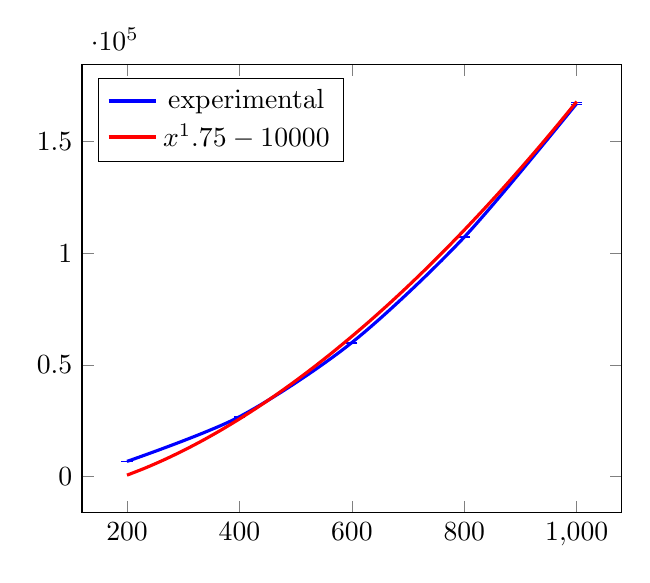
\begin{tikzpicture}
\begin{axis}[legend pos=north west]
\addplot+[line width=0.4mm,smooth,mark=,error bars/.cd, y dir=both,y explicit ]
    coordinates {
        (200, 6789.077        ) +- (55.94397912        ,55.94397912        )
        (400, 26776.464        ) +- (115.4145624        ,115.4145624        )
        (600, 59975.382        ) +- (181.7416356        ,181.7416356        )
        (800, 107165.526        ) +- (244.5757769        ,244.5757769        )
        (1000, 166955.155        ) +- (295.6718837        ,295.6718837        )
    };
\addlegendentryexpanded{experimental}
\addplot+[line width=0.4mm,smooth,mark=,domain=200:1000] {(x^1.75) - 10000};
\addlegendentryexpanded{$x^1.75 - 10000$}
\end{axis}
\end{tikzpicture}

Matthew Oliver
\end{document}